%%%%%%%%%%%%%%%%%%%%%%%%%%%%%%%%%%%%%%%%%%%%%%%%%%%%%%%%%%%%%%%%%%%%%%%%%%%%%%%%%%%
%%%%%%%%%%%%%%%%%%%%%%%%%%%%%%%%%%%%%%%%%%%%%%%%%%%%%%%%%%%%%%%%%%%%%%%%%%%%%%%%%%%
%%%%%%%%%%%%%%%%%%%%%%%%%%%%%%%%%%%%%%%%%%%%%%%%%%%%%%%%%%%%%%%%%%%%%%%%%%%%%%%%%%%
\documentclass[10pt]{beamer}
\usepackage{amsmath}
\usepackage{bm}
\usepackage[english]{babel}
\usepackage{times}
\usepackage[T1]{fontenc}
\usepackage{xmpmulti}

\setbeamercovered{highly dynamic}

\newcounter{saveenumi}
\newcommand{\seti}{\setcounter{saveenumi}{\value{enumi}}}
\newcommand{\conti}{\setcounter{enumi}{\value{saveenumi}}}


\def\vec#1{\text{\bfseries{\rmfamily{#1}}}} 
%\setbeamertemplate{navigation symbols}{} 

\mode<presentation>
{
  \usetheme{Copenhagen}
  \useinnertheme{circles}
  \usecolortheme{dolphin}
  \usecolortheme[rgb={0,0.2,0}]{structure}  
  \usefonttheme[onlymath]{serif}
}

\title[Surface Emission from Neutron Stars\qquad \qquad \ \insertframenumber/\inserttotalframenumber]{Surface Emission from Neutron Stars}

\subtitle{and Implications for the Physics of their Interiors, \\based on F. Ozel, arXiv:1210.0916}
\author[Marina von Steinkirch]{Marina von Steinkirch} 
\institute[SUNY Stony Brook]
{
  Department of Physics \& Astronomy\\
  State University of New York at Stony Brook\\
}
\date{\scriptsize{Astro Journal Club, 10/19/2012}}


%%%%%%%%%%%%%%%%%%%%%%%%%%%%%%%%%%%%%%%%%%%%%%%%%%%%%%%%%%%%%%%%%%%%%%%%%%%%%%%%%%%
%%%%%%%%%%%%%%%%%%%%%%%%%%%%%%%%%%%%%%%%%%%%%%%%%%%%%%%%%%%%%%%%%%%%%%%%%%%%%%%%%%%
%%%%%%%%%%%%%%%%%%%%%%%%%%%%%%%%%%%%%%%%%%%%%%%%%%%%%%%%%%%%%%%%%%%%%%%%%%%%%%%%%%%
\begin{document}

\begin{frame}
  \titlepage
\end{frame}

\begin{frame}
\frametitle{Outline of This Talk}  
\begin{columns}[c]
\begin{column}{0.6\textwidth} 
  \tableofcontents
  \end{column}
  \begin{column}{0.55\textwidth} 
  \begin{center}\scriptsize{
  {\bf ANALYTIC EQUATIONS:}\\
  Neutron Star's EoS constrained by (R,M)\\
  
  \quad
  
   
\includegraphics[scale=0.15]{figs/arrow.png}\\
  
  \quad
  
  {\bf OBSERVATIONAL ASTROPHYSICS:}\\
  Many different observables and methods of observation, currently still not precise enough.
  
  \quad
  
   
\includegraphics[scale=0.15]{figs/arrow.png}\\
  
  \quad
  
  {\bf  COMPUTATIONAL SIMULATIONS AND FITTINGS:}\\
  Surface is what you probe: Many theoretical models of atmosphere for many physical parameters.
  }
  \end{center}
\end{column}
\end{columns}

\end{frame}


\section{Physics of  Neutron Stars (NS)}


\begin{frame}
\begin{center}
 
	{\bf  ANALYTIC EQUATION OF STATE}
\end{center}

\end{frame}

\subsection*{Neutron Stars Overview}
\begin{frame}
\frametitle{Neutron Stars Overview}  
\begin{columns}[c]
\begin{column}{0.65\textwidth} 
\begin{enumerate}
\scriptsize{
 \item Objects with {\bf most extreme densities ($\rho$)}  and {\bf strongest magnetic field (B)}.
 
 \quad
 
 \item  {\bf Energetically favorable} for protons and electrons to form {\bf free neutrons}, generating the {\bf degeneracy pressure}.\\ {\tiny (but core exhibits collective behavior of particles)}
% Free neutrons normally $\beta$ decay in $\sim 15$ minutes, but at sufficient depths in the NS the decay reaction is suppressed as the Fermi energy becomes too high to be populated by the electrons which would be created in the decay. 
 
 \quad
  
 
\item Observations of NSs constrain the physics of their {\bf interiors}:
\begin{itemize}\scriptsize{
 \item {\bf low temperatures},
 \item $\rho \gg$ {\bf  nuclear saturation density}. \\{\tiny ($\rho_s \sim 2.7 \times 10^{14}$ g cm$^{-3})$}}
\end{itemize}

  \quad
  
 
 \item {\bf Photons emitted} from the NS {\bf surface} are direct probes of their {\bf structure, composition, and magnetic field}.
 
 \quad
 
 \item Determining the {\bf EoS} of this {\bf cold ultradense matter} is a {\bf challenge} of high-energy and nuclear astrophysics!

 }
 
\end{enumerate}
\end{column}
\begin{column}{0.5\textwidth}    
 \center{\tiny QCD phase diagram:\\
 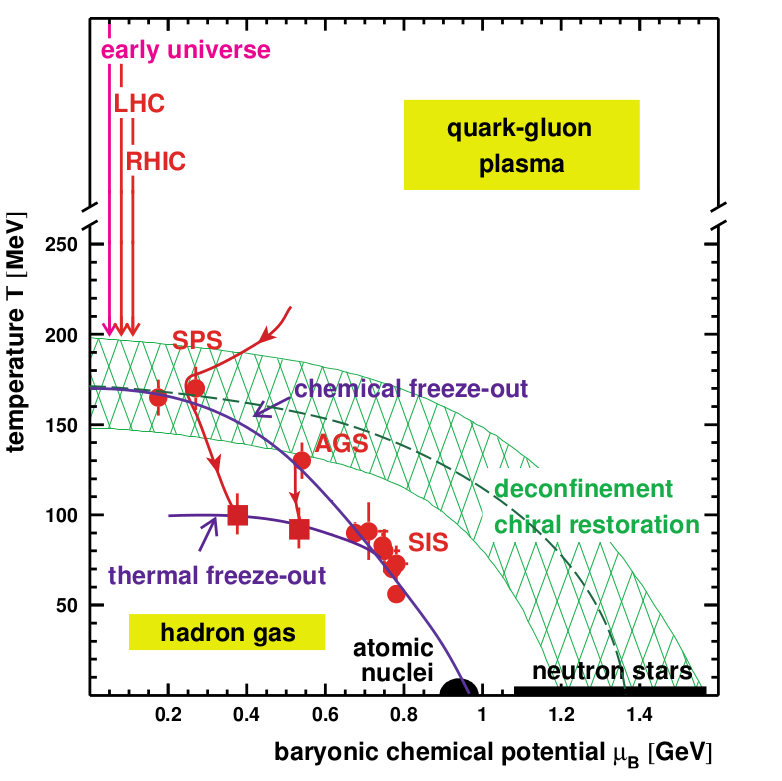
\includegraphics[scale=0.2]{figs/phasetran.png}\\
 High-density/low T region is inaccessible to terrestrial \\experiments (Paerels et al, 2009).}
\end{column}
\end{columns} 
\end{frame}






%%%%%%%%%%%%%%%%%%%%%%%%%%%%%%%%%%%%%%%%%%%%%%%%%%%%%%%%%%%%%%%%%%%%%%%%%%%%%%%%%%%

\subsection*{Neutron Star Radii and Compactness}
\begin{frame}
\frametitle{Neutron Star Radii and Compactness}

\begin{columns}[c]
\begin{column}{0.55\textwidth}

\begin{itemize}
\scriptsize{
\item  {\bf NS EoS} is hard to be obtained from first principles.

\quad
 
 \item Matter that can only be probed through astrophysical observations of {\bf mass} and {\bf radius} with {\bf sufficient precision}!  \\{\tiny (Lattimer $\&$ Prakash , 2007)}
 
 \quad
 
\item Unique map between microscopic {\bf (P-$\rho$)} and macroscopic {\bf(M-R)}.


\quad

\item For instance, $M_{NS}=1.4 M_{\odot}$ gives determination of pressure at $2 \rho_s$.\\ {\tiny (Lattimer $\&$ Prakash , 2011)}
}


\end{itemize}
\end{column}

\begin{column}{0.6\textwidth}
 \center{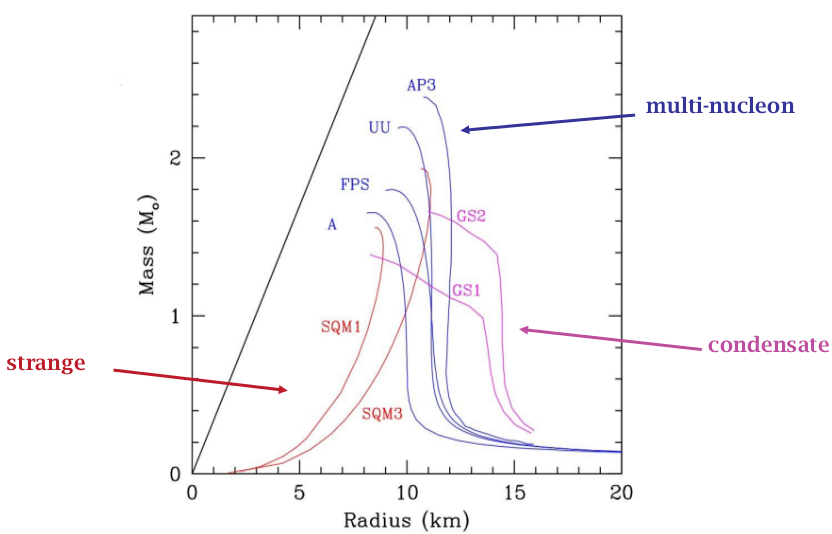
\includegraphics[scale=0.2]{figs/oz.png}}\\
	{\tiny {\bf Mass-radius relations for a selection of NS EoS}: \\{\bf APR} (Akmal et al., 1998), {\bf MS} (M\"uller \& Serot, 1996), {\bf GS} (Glendenning \& Schaffner-Bielich, 1999), {\bf  ABPR }(Alford et al., 2005),  {\bf BBB} (Brueckner-Hartree-Fock model), {\bf SQM }(Prakash et al., 1995).}
 \end{column}
 \end{columns}
\end{frame}



%%%%%%%%%%%%%%%%%%%%%%%%%%%%%%%%%%%%%%%%%%%%%%%%%%%%%%%%%%%%%%%%%%%%%%%%%%%%%%%%%%%


\subsection*{How to Obtain R and M?}
\begin{frame}
\frametitle{Some Initial Quantities to infer (M,R)}

\begin{columns}[c]
\begin{column}{0.6\textwidth} 

\begin{enumerate}\scriptsize{
\item Observational appearance of NS affected by {\bf redshift and lensing effects}.

\quad



\item The {\bf redshift} is
$$1+z = |g_{tt}|^{-1/2} = \Big(1 - \frac{2GM}{Rc^2} \Big)^{-1/2}.$$



\item The apparent radius at some distance $D$ is then
$$R_{\infty} = R \Big( 1 - \frac{2GM}{Rc^2}\Big)^{-1/2}.$$



%\item (M-R) relation are given by $R = R_{\infty} (1 + z) -1 ,$
%$M = R_{\infty} c^2 (1 + z)-1= [1 - (1 + z)^{-2} ]/2G.$

\item {\bf Lensing} from a {\bf strong gravitational field} gives an area which  appears to be large by 
$$\frac{S_{\infty}}{4\pi R^2} = (1+z)^2.$$


}
\seti
\end{enumerate}
\end{column}
\begin{column}{0.6\textwidth} 
\begin{enumerate}\scriptsize{
\conti


%\item The {\bf  Eddington luminosity at infinity } is:
%$L_{E,\infty} = \frac{8\pi m_pc}{(1+X)\sigma_T} \Big (1 - \frac{2GM}{Rc^2} \Big)^{1/2}.$

\item The {\bf  total flux } observed at distance $D$ is 
$$F_{\infty} = \sigma_B T^4_{eff,\infty} \Big ( \frac{R}{D} \Big)^2 (1+z)^2.$$


\item  Uncertainties given by:
\begin{itemize}\scriptsize{
 \item {\bf distance} ($R_{\infty} \propto D$),
 \item  {\bf interstellar H absorption},
 \item and {\bf atmospheric composition}. }
\end{itemize}

\quad

\item {\bf Best probes}: 
\begin{itemize}\scriptsize{
 \item nearby isolated NS (parallax measurable),
 \item and X-ray binaries in globular clusters.
}\end{itemize}

}
\end{enumerate}
 \end{column}
 \end{columns}
\end{frame}




%%%%%%%%%%%%%%%%%%%%%%%%%%%%%%%%%%%%%%%%%%%%%%%%%%%%%%%%%%%%%%%%%%%%%%%%%%%%%%%%%%%

\subsection*{Energy Sources in Neutron Stars}

\begin{frame}
\frametitle{Energy Sources in Neutron Stars:}  
\begin{enumerate}
 \item Radiation of Residual Heat in Young NSs.
 
 \quad
 
 \item Re-radiation of deposition heat between accretion episodes.
 
 \quad
 
 \item Magnetic Field Decay.
 
 \quad

 \item Particle Bombardment onto Polar Caps.
 
  \quad
 
 \item {\bf Thermonuclear Bursts}.
 
\end{enumerate}
\end{frame}







%%%%%%%%%%%%%%%%%%%%%%%%%%%%%%%%%%%%%%%%%%%%%%%%%%%%%%%%555



\section{Physics of NS Surface Emission}





%%%%%%%%%%%%%%%%%%%%%%%%%%%%%%%%%%%%%%%%%%%%%%%%%%%%%%%%%%%%%%%%%%%%%%%%%%%%%%%%%%%


\begin{frame}
\begin{center}
 
	{\bf  OBSERVATIONAL ASTROPHYSICS} 
\end{center}

\end{frame}


\subsection*{Observing Neutron Stars and their Surfaces} 

\begin{frame}
\frametitle{Observing Neutron Stars and their Surfaces} 

\begin{columns}[c]
\begin{column}{0.55\textwidth} 
	{\bf \center We probe NSs from:}{\scriptsize
	 \begin{enumerate}
	     \item Dynamics of {\bf binary systems}.
	     \item Structure and energetics of {\bf radio pulse sources}.
	     \item {\bf Spectra and variability} of their high energy radiation.
	     \item {\bf Direct observations} of the {\bf  surface emission} (often hidden from view).
	     	    \end{enumerate}
}
\end{column}
\begin{column}{0.55\textwidth}    
{\bf \center We see evidences of NS surface emission from:}
\begin{itemize}\scriptsize{
		 \item {\bf Thermonuclear bursters from (LMXB)}.
		 \item {\bf Accreting sources during quiescence}. {\tiny
		 \item Isolated cooling NS (DINS), central compact objects (CCO).
		 \item Pulsating sources in radio (PSR).
		 \item Accretion powered pulsars (AMSP) and accreting millisecond X-ray pulsars (MSP), Soft gamma-ray repeaters(SGR), anomalous X-ray pulsars (AXP).}}
	  \end{itemize}
	  \end{column}
\end{columns}
 \center{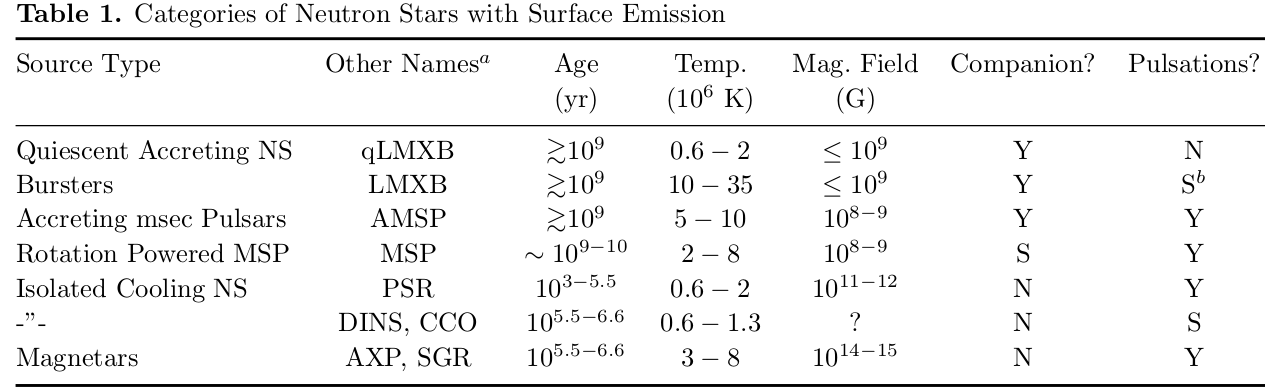
\includegraphics[scale=0.19]{figs/all.png}}

\end{frame}



%%%%%%%%%%%%%%%%%%%%%%%%%%%%%%%%%%%%%%%%%%%%%%%%%%%%%%%%%%%%%%%%%%%%%%%%%%%%%%%%%%%

\subsection*{Neutron Star Sources with Surface Emission}
\begin{frame}
\frametitle{Neutron Star Sources with Surface Emission}
\center{ {\bf Surface emission}  detected in many NS sources, with {\bf thermal spectra from optical to X-rays}: }

\begin{columns}[c]
\begin{column}{0.5\textwidth} 
 \scriptsize{
 \item {\bf Accreting NS in quiescence:} \\
 
 \quad
 
 \begin{itemize}\scriptsize{
 \item  Half of NS accreting from low-mass companion have X-ray transients.
 
 
 
 \quad
 
  \item {\bf X-rays transients} have several different accretion phases, varying flux level and spectral characteristics.
  
  \quad
  
  \item {\bf Outburst luminosity} $\sim 10^{36-38}$ erg s$^{-1}$, same order of their {\bf quiescent luminosity}.}
 \end{itemize}}

 


\end{column}
\begin{column}{0.65\textwidth}   

 \scriptsize{
 
\item {\bf Accreting Bursting NS (from LMXB):}\\

\quad

\begin{itemize}\scriptsize{

\item 100 of $\sim$ 150 exhibit thermonuclear bursts, with X-ray flux rising $\sim 10-100$ s.

\quad

 \item Due to {\bf unstable burning of He/H}, {\bf accreted} to the NS surface from companion.
 
 \quad
 
 \item  {\bf Evolution of the color temperature} in the burst: dip in the {\bf T} rises {\bf photospheric radius expansion} (PRE).
 

 
 }
 
 
\end{itemize}
} 

\end{column}
\end{columns}
\end{frame}


%%%%%%%%%%%%%%%%%%%%%%%%%%%%%%%%%%%%%%%%%%%%%%%%%%%%%%%%%%%%%%%%%%%%%%%%%%%%%%%%%%
\subsection*{Type I X-Ray Bursters and LMXBs  }
\begin{frame}
\frametitle{Type I X-Ray Bursters and LMXBs}

\begin{columns}[c]
\begin{column}{0.6\textwidth} 
\begin{enumerate}\scriptsize{
\item {\bf X-ray bursters} (XRB) are periodic and rapid increases in luminosity in the X-ray range.

\quad


\item XRB are composed of {\bf an accreting compact object} (NS) and a {\bf companion}, whose mass categorizes the system:
\begin{itemize}\scriptsize{
 \item High mass ($M > 10 M_{\odot}$), {\bf (HMXB)}.
 \item Low mass ($M < 1 M_{\odot}$), {\bf (LMXB)}.}
\end{itemize}

\quad

\item {\bf Low mass X-ray Bursters} (LMXB) are {\bf thermonuclear} XRB that can put constraints on the NS EoS.

\quad

 
 \item For instance, observations of {\bf NS during thermonuclear bursts} have led to the {\bf  first constraining measurements of NS radii}: \\9 km $<$ R $<$ 12 km. \\{\tiny (Lattimer $\&$ Brown, 2010)}


}
\end{enumerate}
\end{column}
\begin{column}{0.55\textwidth}

  \center{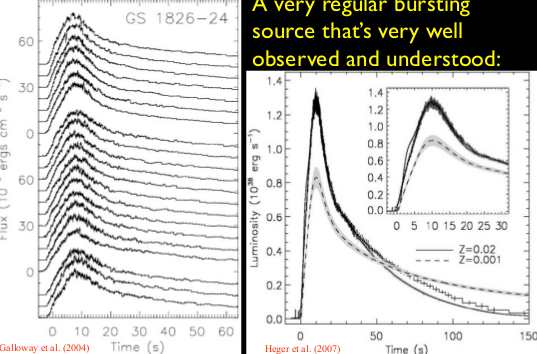
\includegraphics[scale=0.33]{figs/xx.png}}
\end{column}
\end{columns}
\end{frame}





%%%%%%%%%%%%%%%%%%%%%%%%%%%%%%%%%%%%%%%%%%%%%%%%%%%%%%%%%%%%%%%%%%%%%%%%%%%%%%%%%


\subsection*{Photospheric Radius Expansion (PRE) Bursts}
\begin{frame}
\frametitle{Photospheric Radius Expansion (PRE)}

\begin{columns}[c]
\begin{column}{0.55\textwidth} 

\begin{enumerate}
\scriptsize{
 \item  NS Observations are from the outermost layer of surface, the {\bf photosphere}, in radioactive equilibrium given by a flux 
$F=\sigma_B T^4_{eff}.$
 
 \quad

\item {\bf PRE bursts} are a {\bf bright} subset of TB where  at the so-called {\bf touchdown point} (where the {\bf photosphere} returns to the NS radius), fluxes are close to $L_{Edd} = 4 \pi R^2 \sigma_T T^4_{eff}.$ on the surface.

\quad

\item  $F_{Edd}$ can be related to the {\bf normalization of the burst spectrum} (blackbody normalization, $K$),  which gives the  {\bf emitting area} (R):


$$F_{Edd} = F_{touchdown} = \frac{GMc}{\kappa D^2} \Big ( 1 - \frac{2GM}{Rc^2} \Big)^{1/2},$$
$$ A = \frac{R^2}{D^2f_c^4} \Big( 1 - \frac{2GM}{Rc^2} \Big )^{-1} = f_c  K^{1/4},$$
 $f_c$ the color correction factor.


 }
  \end{enumerate}
  
  

\end{column}
\begin{column}{0.7\textwidth}
\begin{center}
\scriptsize{
Debate about {\bf systematic errors} that must be taken\\ into account ({\bf where is the touchdown?}). }
\\{\tiny (Suleimanov et al. 2011a; Guver, Ozel $\&$ Psaltis 2011)} 

\quad

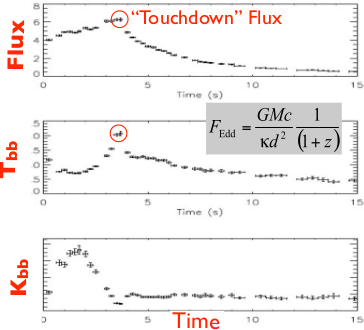
\includegraphics[scale=0.45]{figs/pree.png}
\end{center}

\quad 
  \end{column}
\end{columns}
   \end{frame}
   
   
 
 

\begin{frame}
\begin{center}
 
	{\bf  COMPUTATIONAL SIMULATIONS\\ AND FITTINGS} 
\end{center}

\end{frame}



\section{Modeling NS Atmospheres}

\subsection*{Parameters for Modeling Neutron Star Atmospheres}

\begin{frame}
\frametitle{Parameters for Modeling Neutron Star Atmospheres}

\begin{center}
 

	Detailed {\bf Models of NS atmospheres} shape the {\bf spectrum } and {\bf pattern of radiation} from {\bf crust and core}. 


\end{center}

	\begin{itemize}

	\item 
Assumptions:
\begin{enumerate}
 \item {\bf Plane-parallel} geometry.
 \item {\bf Radioactive equilibrium}.
 \item {\bf Hydrostatic equilibrium}.
\end{enumerate}
\quad

	 \item The {\bf four parameters} in the models are:
	   \begin{enumerate}
	    \item Magnetic field strengths;
	    \item Chemical Compositions (e.g. H fraction, $X$);
	    \item Temperature at surface, $T_{eff}$;
	    \item Gravitational acceleration at surface, $g$.
	   \end{enumerate}
	\end{itemize}	   
\end{frame}





%%%%%%%%%%%%%%%%%%%%%%%%%%%%%%%%%%%%%%%%%%%%%%%%%%%%%%%%%%%%%%%%%%%%%%%%%%%%%%%%%%%


\subsection*{Modeling the Spectrum of the  NS Surface Emission}



\begin{frame}
\frametitle{Some Results on Modeling and Fitting Spectra}
\begin{columns}[c]
\begin{column}{0.7\textwidth} 
\begin{enumerate}
\scriptsize{
\item Many different {\bf physical conditions}: {\tiny ( Suleimanov et al, 211)}
\begin{itemize}\scriptsize{
 \item 6 different {\bf chemical compositions} (pure H, pure He, solar mix, heavy elements).
 \item 3 values of {\bf surface gravities}.
 \item 20 values of {\bf luminosities} in units $l = L/L_{Edd}$.}
\end{itemize}

\quad
 
\item {\bf NS spectra} look like blackbody, but shifted to higher temperatures by the {\bf color coefficient factor}:
$$f_c = \frac{T_{BB}}{T_{eff}} = K^{-1/4}A $$

\item Fitting $f_cT_{eff}-l$ to the $K^{-1/4}-F_{\infty}$ on cooling LXRB  at some $D$, gives $$R_{\infty}=R(1+z)=R_{BB} f_c^2.$$ 

\quad

\item {\bf Others processes considered}: angular redistribution in scattering, electron conduction, {\bf Compton scattering}...
}
\end{enumerate}
\end{column}
\begin{column}{0.5\textwidth} 

 \center{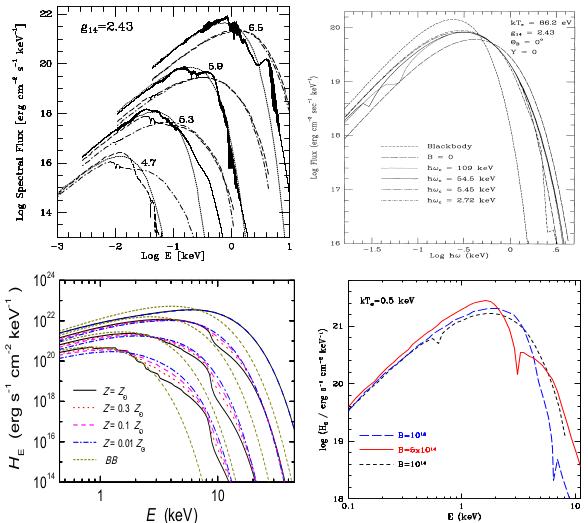
\includegraphics[scale=0.23]{figs/atms.png}}\\
 {\tiny Model spectra for four different types of NS, $H_E=4\pi H_E$: non-magnetic cool NS, cool with moderate B, hot bursting with mentalities, strong B with H.}

 \end{column}
 \end{columns}

\end{frame}


%%%%%%%%%%%%%%%%%%%%%%%%%%%%%%%%%%%%%%%%%%%%%%%%%%%%%%%%%%%%%%%%%%%%%%%
\subsection*{Some Results on Modeling and Fitting Spectra}

\begin{frame}
\frametitle{Results on Modeling and Fitting NS Spectra}
\begin{columns}[c]
\begin{column}{0.55\textwidth} 
 \center{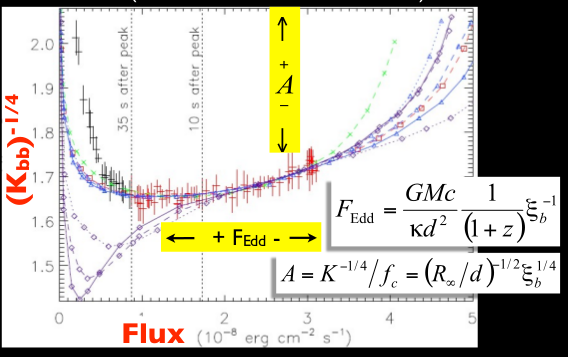
\includegraphics[scale=0.3]{figs/qqq.png}}\\
 {\tiny (Suleimanov et al, 2011)}\\
 

\end{column}
\begin{column}{0.55\textwidth} 
 \center{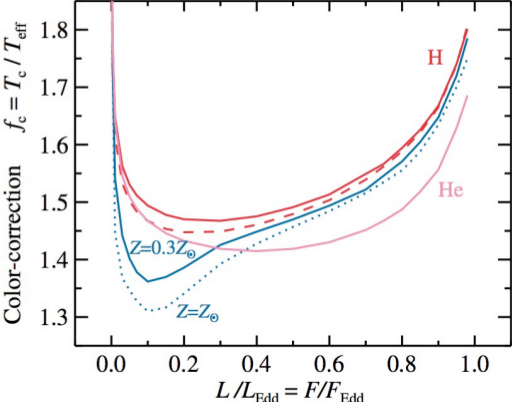
\includegraphics[scale=0.3]{figs/meu.png}}
  {\tiny (October/2012)}
 \end{column}
 \end{columns}
 
\end{frame}




\begin{frame}
\begin{center}
 
	{\bf  OUTLOOK}
\end{center}

\end{frame}


\section{Outlook}

\subsection*{State of Art and Future}
\begin{frame}
\begin{columns}[c]
\begin{column}{0.55\textwidth} 
{\bf \center State of Art:}

\quad

\begin{enumerate}
\scriptsize{
 \item Measuring different {\bf NSs (M-R)} can {\bf constrain the EoS} of cold ultradense matter.
 
 \quad
 
 \item  More than 10 years worth of {\bf Rossi X-ray Timing Explorer}(RXTE), the {\bf Chandra X-ray Observatory}, and the {\bf XMM-Newton observations}, with many NSs showing {\bf thermal emission}.
 
 \quad
 
  \item {\bf X-ray bursts}  useful for inferring {\bf NSs (M-R)}, but systematic and statistical errors  {\bf currently do not allow to pin down a unique EoS}. 
  
}
\end{enumerate}
\end{column}

\begin{column}{0.55\textwidth}  
{\bf \center Future Missions and Challenges:}
\begin{enumerate}\scriptsize{
 \item Future observations with {\bf high spectral energy resolution}: {\bf Astro-H}, {\bf ATHENA}.
 

   
 \quad
 
 \item {\bf GAIA} mission will allow {\bf precise measurements of source distances}, constraining $D$ for the radius determination of {\bf thermally emitting stars}.
 
 
 
 \quad
 
 \item Observations of NSs with {\bf  high timing resolution} will be possible with {\bf LOFT} mission.
 
 \quad
 
 \item  {\bf Other approaches to constrain (M-R)} can be explored, e.g. modeling the {\bf pulse profiles} from {\bf non-uniform emission from surface of rotating NSs}, looking for primary {\bf GR effects}.
 

 
 \quad
 
 \item Achieving  {\bf overconstrained measurements} in the EoS allows testing {\bf effects of strong gravitational fields} on NS surfaces.
 }
\end{enumerate}
\end{column}

\end{columns}
\end{frame}





%%%%%%%%%%%%%%%%%%%%%%%%%%%%%%%%%%%%%%%%%%%%%%%%%%%%%%%%%%%%%%%%%%%%%%%%%%%%%%%
%%%%%%%%%%%%%%%%%%%%%%%%%%%%%%%%%%%%%%%%%%%%%%%%%%%%%%%%%%%%%%%%%%%%%%%%%%%%%%%
%%%%%%%%%%%%%%%%%%%%%%%%%%%%%%%%%%%%%%%%%%%%%%%%%%%%%%%%%%%%%%%%%%%%%%%%%%%%%%%
\subsection*{Backup}

\begin{frame}
\frametitle{What are X-ray bursts}
\begin{itemize}\scriptsize{
 \item More than 2000 NSs have been discovered in the Galaxy, from {\bf pulsating sources in radio} to {\bf bright persistent sources in X-Rays}.
 
 \quad
 
 \item They are {\bf bright}.
 
 \quad 
 
 \item We see the {\bf neutron star surface}.
 
 \quad
 
 \item Spectra well fit by {\bf Planck curves}.
 
 \quad
 
 \item {\bf Type I X-ray bursts} to infer {\bf (M,R)}.
 
 \quad
 

\item The large observational catalogues of type I X-ray bursts now available.
}
\end{itemize}
\end{frame}





%%%%%%%%%%%%%%%%%%%%%%%%%%%%%%%%%%%%%%%%%%%%%%%%%%%%%%%%%%%%%%%%%%%%%%%%%%%%%%%%%%%


\begin{frame} 
\begin{columns}[c]
\begin{column}{0.65\textwidth} 
	{\bf \center Radiation of Residual Heat in Young NSs} 
\begin{enumerate}
\scriptsize{
	   \item {\bf After Supernova explosion}: 
	   \begin{itemize}\scriptsize{
	    \item Hot protoneutron star with $T\sim 10^{11} K$;
	    \item Cools by $\nu$ emission from the interior to surface.}
	   \end{itemize}

	   
	   \item {\bf After the supernova explosion}: 
	   \begin{itemize}\scriptsize{
	    \item NS divided into a stellar interior and an outer heat blanketing envelope;
	    \item The interior becomes isothermal within few years.
	    \item The envelope sustains strong $\nabla \textbf{ T}$, is $\sim 100$ m deep, and has short time relaxation, stationary, plane-parallel in hydrostatic equilibrium.
	      \item The thermal evolution of the core (described by the GR solutions of a spherical symmetric star) depends on the heat capacity (degenerate constituents) of the core and neutrino emissivity (composition).}
	   \end{itemize}

	  
	   \item {\bf First 10-100 years}: stellar envelope thermally relaxes by radiating its thermal energy.
	   
	   \quad
	   
	   \item {\bf Following $10^5$ years}: temperature of the crust is set by the temperature of the isothermal core.
	   }
\end{enumerate}	
\end{column}
\begin{column}{0.4\textwidth}    
 \center{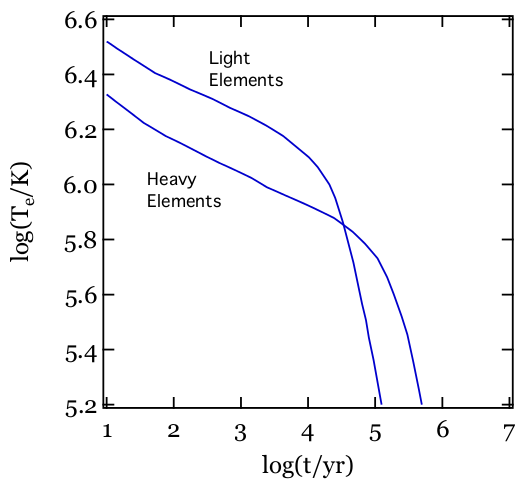
\includegraphics[scale=0.23]{figs/cool.png}}\\
 {\tiny Thermonuclear burst from 4U 1636+536 showing PRE (a) compared to an ordinary burst in panel (b). }
\end{column}
\end{columns}
\end{frame}





%%%%%%%%%%%%%%%%%%%%%%%%%%%%%%%%%%%%%%%%%%%%%%%%%%%%%%%%%%%%%%%%%%%%%%%%%%%%%%%%%%%

\begin{frame}
\begin{columns}[c]
\begin{column}{0.5\textwidth} 
	{\bf \center Reradiation of deposition heat between accretion episodes:}

	
 	{\scriptsize 
	  \begin{itemize}
	   \item Electron capture and pycnocuclear reactions at $\rho \sim 10^{12}$ g cm$^{-3}$ at the crust, releasing $Q_{nuc} \sim 1.5-2$ MeV per accreted baryon.
	   
	   \quad
	   
	   \item A fraction of energy missed by neutrino radiation but some is deposit in the interior, sufficient to power quiescent emission.
	  \end{itemize}
	}    
\end{column}
\begin{column}{0.5\textwidth}  
	{\bf \center Magnetic Field Decay:}
	

 	{\scriptsize 
	  \begin{itemize}
	  \item Decay of strong B $(>10^{14}$ G) releases hot from crust fracturing under stress. {\tiny (Cumming et al 2008, Arras et al, 2004)}
	  
	  \quad
	  
	  \item $E\sim 10^{44}$ erg over hundred section.
	  \end{itemize}
	}   
	\quad
	
		{\bf \center Particle Bombardment onto Polar Caps:}
		
		
 	\scriptsize{ Relativistic electron-positron in the magnetosphere of pulsar bombard the polar caps on the surface, thermal emission peaked in the UV to X-ray. }


\end{column}
\end{columns}
\end{frame}

%%%%%%%%%%%%%%%%%%%%%%%%%%%%%%%%%%%%%%%%%%%%%%%%%%%%%%%%%%%%%%%%%%%%%%%%%%%%%%%%%%%


\begin{frame}

\begin{columns}[c]
\begin{column}{0.5\textwidth} 
	{\bf \center Surface Composition}

\begin{itemize}\scriptsize{ 
 \item Composition of NS determined by: abundance of material during supernova explosion, abundance of material accreted from companion or ISM, gravitational ?? of heavy elements.
 \item Even  light elements like O can remain in the photosphere and give atomic lines on the spectrum  if there is no lighter elements or if its continuously fueled by accretion or convection (short timescale for sedimentation of heavy elements).
 \item The amount of H to cover the surface of a NS down to its photosphere (non B) is
 $$ M_H = 4 \pi R^2 h N_p m_p,$$
 with gas ionized ($N_H=N_p$), which shows to be very small, and the timescale for accretion of sufficient H to cover surface $\ll$ 1 yr to $\sim 10^3$ yr, dominant H and He.}
 \end{itemize}

\end{column}
\begin{column}{0.5\textwidth} 
 
 	{\bf \center  Magnetic Field Strengths}
 \begin{itemize}\scriptsize{ 
  \item From $<10^8$ G to steadying accreting NS to $\sim 10^{15}$ magnetars.
  \item Profound effects on the surface, most important parameter for emission properties.
  \item Affects propagation of photons in the atmosphere, together with polarization of magnetic vacuum (plasma density low)
  \item Photos interact primary  with virtual pairs, vacuum polarization is affected by B, in the presence of a plasma with density gradient (ns atm): resonance on the normal modes of photon propagation, from circular at high e dens (deeper atm) to linear (low densities), so critical density depending on the photon energy, the conversion of photons between the two polarization modes is enhanced, together by chance in the opacities of the normal modes., resonances five rise to broad absorption-like feature. {\tiny (Ozel 2001)}}
 \end{itemize}
 \end{column}
 \end{columns}
\end{frame}




%%%%%%%%%%%%%%%%%%%%%%%%%%%%%%%%%%%%%%%%%%%%%%%%%%%%%%%%%%%%%%%%%%%%%%%%%%%%%%%%%%%




%%%%%%%%%%%%%%%%%%%%%%%%%%%%%%%%%%%%%%%%%%%%%%%%%%%%%%%%%%%%%%%%%%%%%%%%%%%%%%%%%%%


\begin{frame}
\frametitle{Flux and Spectrum of NSs Surface Emission}
\begin{itemize}\scriptsize{ 
 \item Initially the energy is in the crust or core, deeper than atmosphere.
 
 \quad
 
 \item Modeling: assumption of hydrostatic equilibrium, valid if the flux of radiation emitted from the NS does not lead to force $>$ the gravitational force on surface (As long as  the radioactive flux remains below the EL, there is hydrostatic equilibrium).
 
 \quad 
 
 \item Defining {\bf local Eddington limit (EL)} as the luminosity at which radiation balances gravitational forces:
 $L_{Edd} = \frac{8 \pi G M m_p c}{(1+X)\sigma_T}$
 
 \quad
 
\item Very large gravitational acceleration on the NS surface:
$$ g \sim \frac{GM}{R^2} \sim 1.9 \times 10^{14} \Big ( \frac{M}{1.4 M_{cdot}} \Big ) \Big ( \frac{R}{10 m} \Big)^{-2} cm s^{-2}.$$

\item This leads to a very small {\bf scale height} for atmosphere (matter taken as fully ionized):
$$ h \sim 2 \frac{k_BT}{m_p g} \sim 8.8 \Big ( \frac{T}{10^7 K} \Big )  \Big ( \frac{M}{1.4 M_{cdot}} \Big )^{-1} \Big ( \frac{R}{10 m} \Big)^{2} cm.$$

\item Since the scale height $\ll$  NS radius: plane parallel atmosphere in the models.

\quad 


\item 
{\tiny (timescale protons exchange E with matter in photosphere is much shorter than the timescale the interior cools)}

} 
\end{itemize}
\end{frame}



\begin{frame}
\frametitle{Finally, with the right fits...}
\begin{columns}[c]
\begin{column}{0.55\textwidth} 
\begin{center}
  \center{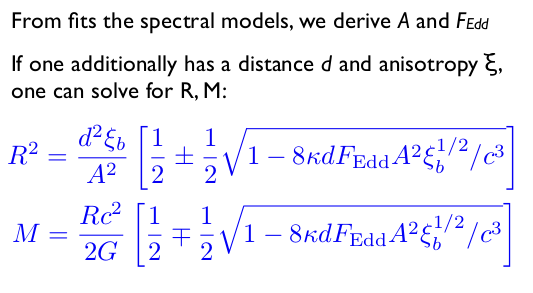
\includegraphics[scale=0.32]{figs/qq.png}}
\end{center}
\end{column}
\begin{column}{0.55\textwidth} 
  \center{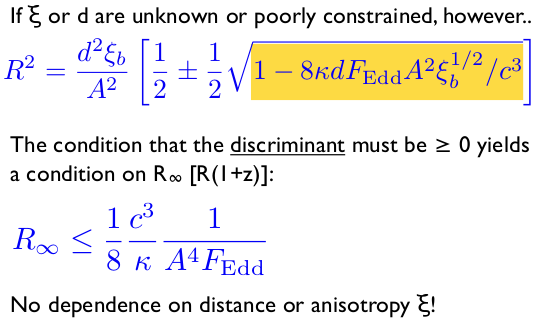
\includegraphics[scale=0.32]{figs/q.png}}
 \end{column}
 \end{columns}

\end{frame}


\begin{frame}
\frametitle{Thermonuclear Bursts (TB)}
	  \begin{enumerate}\scriptsize{ 
	   \item {\bf Recurrent X-ray flashes} with rise time of $\sim 1$ s and duration of $\sim 10$ s  (Type I X-ray bursts, with luminosities up to twice to the {\bf accretion luminosity}).
	   
	   \quad
	   
	      \item Accreting NSs with  {\bf weak B} $(<10^{10}$ G), where {\bf He and H} come from the {\bf binary company}.
	   
	  
	   
	   \quad
	   
	   \item {\bf Several mass accretion rate regimes} leading to thermonuclear flashes with different characteristics. They are typically expressed in units of {\bf Eddington mass accretion rate}:
	  
	  $$\dot M_E = \frac{8 \pi m_p cR}{(1+X)\sigma_T} = 1.8 \times 10^{-8} \Big (\frac{R}{10 \mbox{ km}} \Big ) \Big (\frac{1+X}{1.7}\Big)^{-1} M_{\odot} \mbox{ yr}^{-1}.$$
	  
	where
	  
	  \begin{itemize}\scriptsize{ 
	   \item $\dot m = \dot M/\dot M_E <0.01$: {\bf H burning is unstable and triggers unstable He burning}.
	   \item $0.01< \dot m < 0.1$: {\bf H burns stably into He  between bursts, until He ignites}.
	   \item $0.1< \dot m<0.9$: {\bf He ignites unstably}. }
	  \end{itemize}
}
	  \end{enumerate}
\end{frame}



\end{document}